\documentclass{beamer}
\usepackage[utf8x]{inputenc}
\usepackage[french]{babel} 
\usepackage{lmodern}
\usepackage[T1]{fontenc}
\usepackage{graphicx}
\usepackage{epstopdf}
\usetheme{Hannover}
\title[Phishing-Wlan]{Network 101\\Phishing-wlan}
\author{Authors}
\institute{Institute}
\date{September 21, 2015}
\addtobeamertemplate{footline}{\insertframenumber/\inserttotalframenumber}

\begin{document}

\begin{frame}
	\titlepage
\end{frame}

\AtBeginSubsection[]
{
	\begin{frame}<beamer>
		\frametitle{Layout}
		\tableofcontents[currentsection,currentsubsection]
	\end{frame}
}

\section{Introduction}
\begin{frame}{Introduction}
	\begin{figure}[!h]
		\centering
		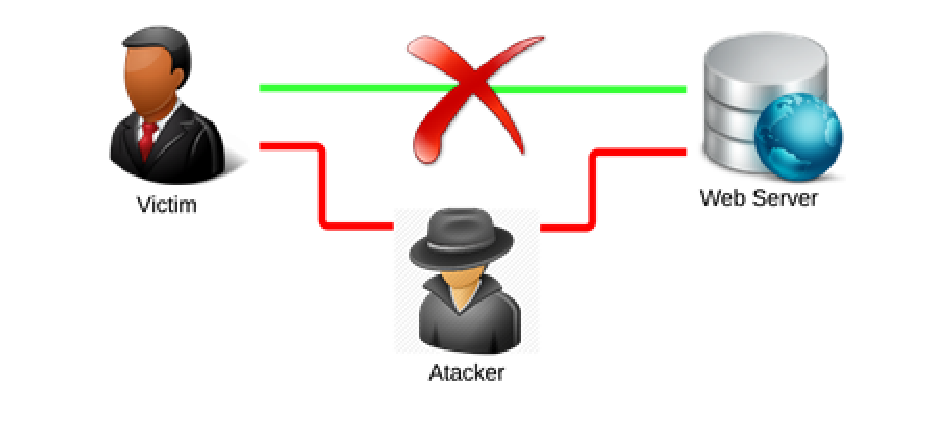
\includegraphics[scale=0.5]{../images/mitm.eps}
		\caption{Man In The Middle attack}
		\label{mitm_attack}
	\end{figure}

    \begin{columns}
		\column{.46\linewidth}
		\begin{itemize}
			\item MITM Attack\\
			\item ARP Spoofing\\
			\item DNS Spoofing\\
		\end{itemize}
		\column{.46\linewidth}
		\begin{itemize}
			\item Steal SSL certificate\\
			\item Steal credentials\\
		\end{itemize}
	\end{columns}
\end{frame}

\section{What we are doing}
\subsection{Global Process}
\begin{frame}{Global Process}
	\begin{figure}[!h]
		\centering
		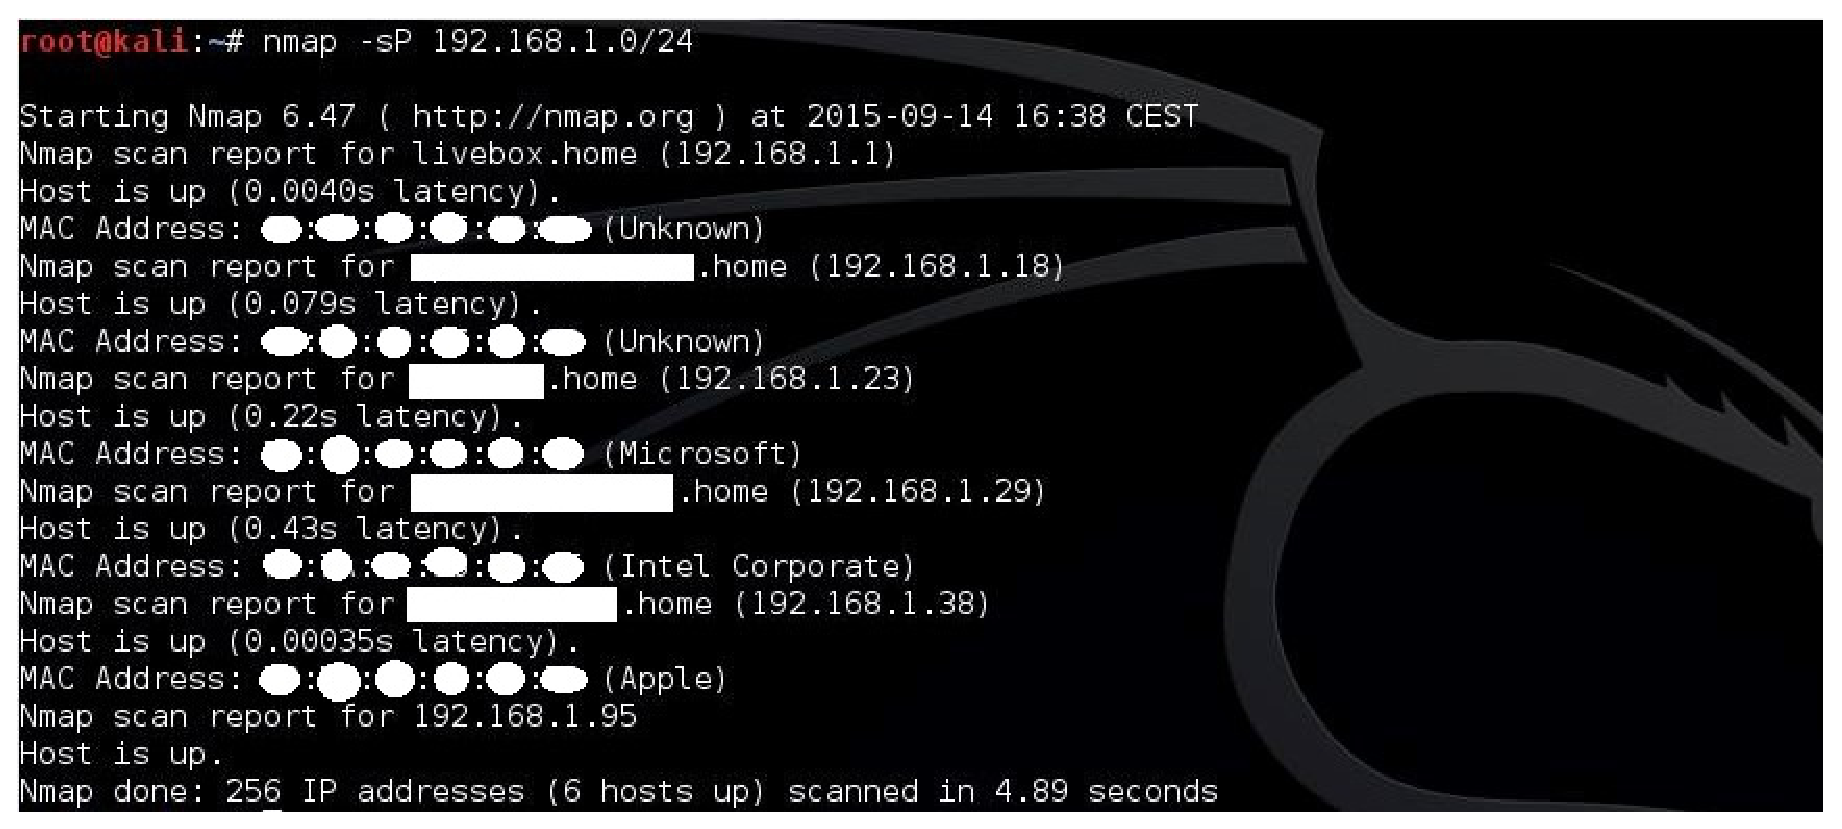
\includegraphics[scale=0.45]{../images/captureNMAP.eps}
		\caption{nmap capture} %la légende
		\label{nmap_capture} %l'étiquette
	\end{figure}
\end{frame}

\subsubsection{ARP Step}
\begin{frame}{ARP Step}
	\begin{figure}[!h]
		\centering
		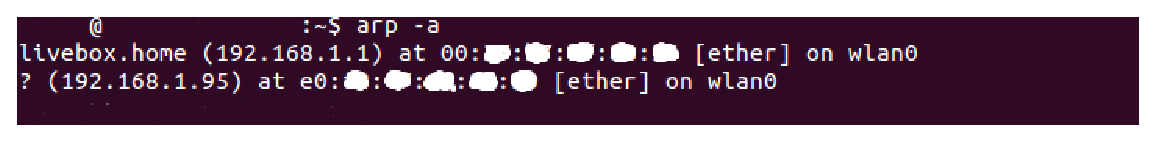
\includegraphics[scale=0.50]{../images/arpTableBeforeSpoof.eps}
		\caption{ARP Table before spoof}
		\label{ARP_before_spoof}
	\end{figure}
	\begin{figure}[!h]
		\centering
		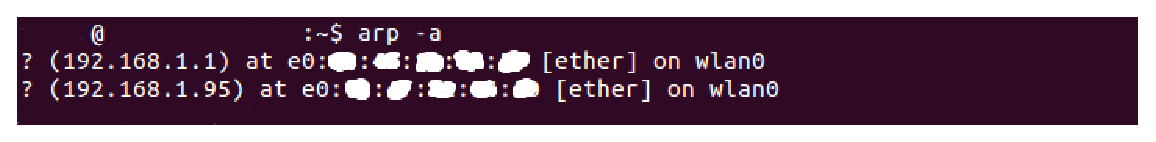
\includegraphics[scale=0.50]{../images/arpTableAfterSpoof.eps}
		\caption{ARP Table after spoof}
		\label{ARP_after_spoof}
	\end{figure}	
\end{frame}

\begin{frame}{ARP spoof message}
	%\begin{center}
		%\begin{verbatim}
			%<MAC_PIRATE> tell <MAC_TARGET> that <IP_GATEWAY> is at <MAC_PIRATE>
		%\end{verbatim}
	%\end{center}

	\begin{figure}[!h]
		\centering
		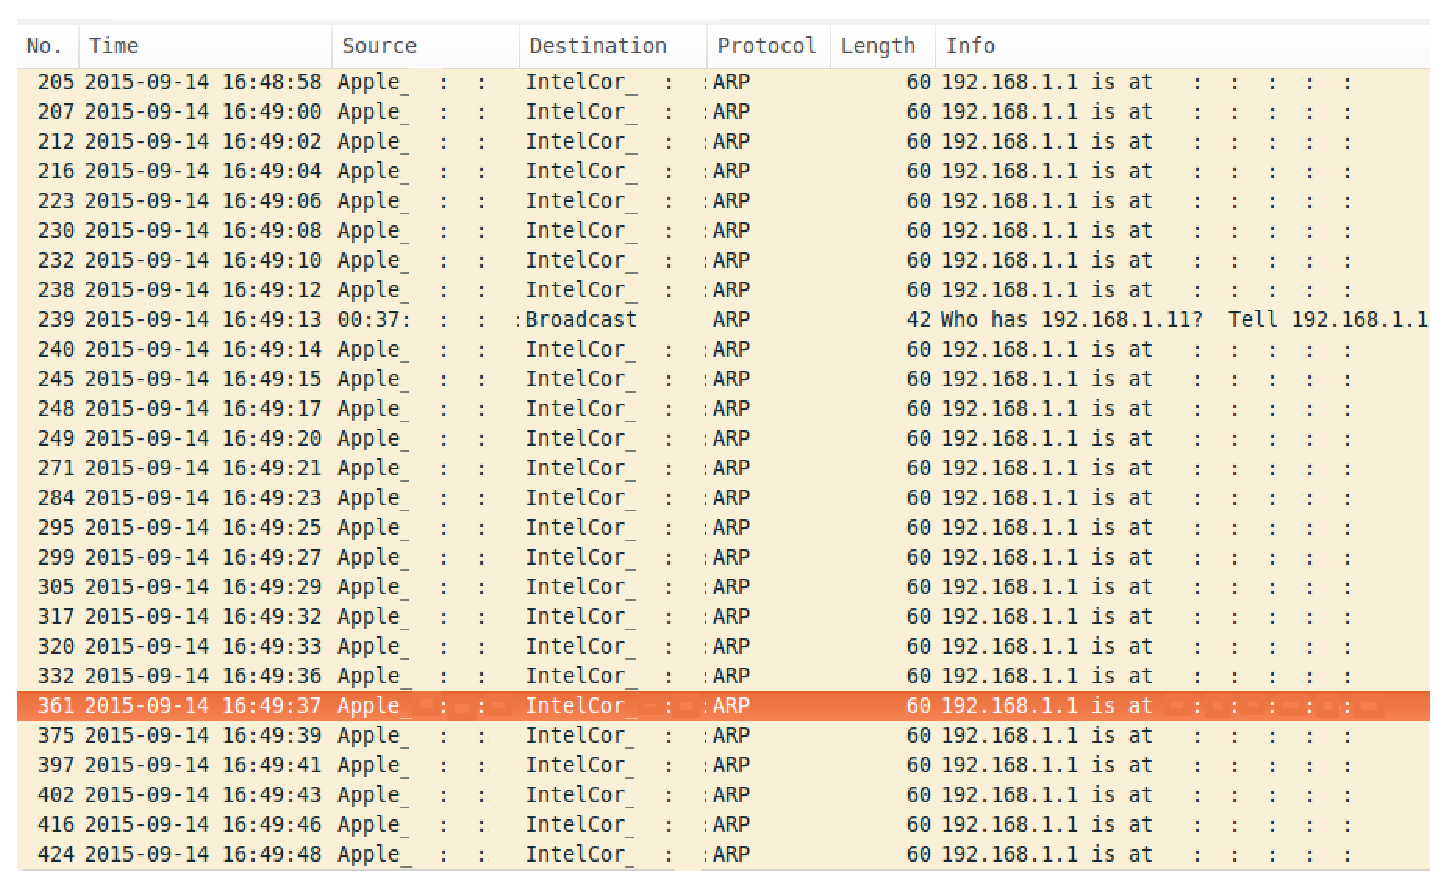
\includegraphics[scale=0.4]{../images/wiresharArpSpoof.eps}
		\caption{Wireshark capture of the ARP spoofing}
		\label{Wireshark_ARP_Spoof}
	\end{figure}
\end{frame}

\subsubsection{DNS Step}
\begin{frame}{DNS Step}
	\begin{figure}[!h]
		\centering
		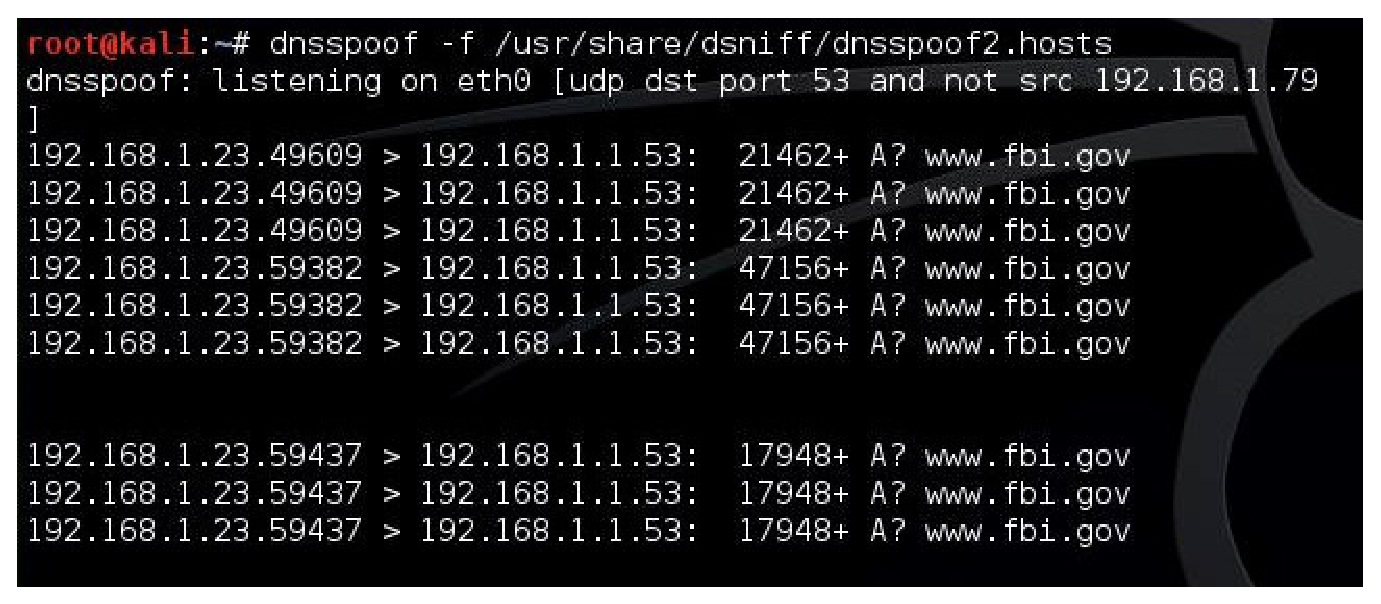
\includegraphics[scale=0.4]{../images/DNSCaptureShell.eps}
		\caption{DNS shell capture}
		\label{DNSCaptureShell}
	\end{figure}
\end{frame}
\begin{frame}{DNS Step}
	\begin{figure}[!h]
		\centering
		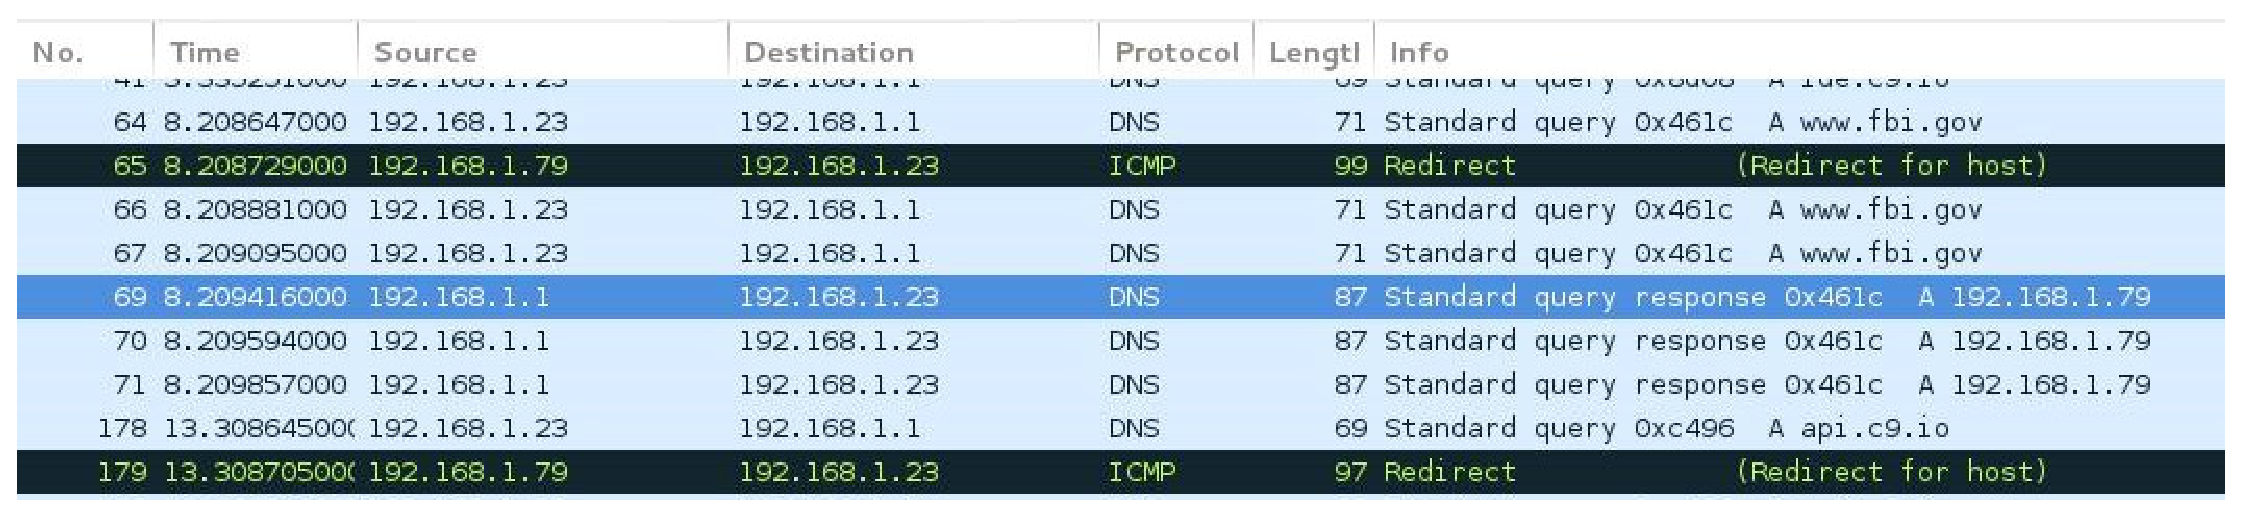
\includegraphics[scale=0.25]{../images/DNSCaptureWireshark.eps}
		\caption{DNS Wireshark capture}
		\label{DNSCaptureWireshark}
	\end{figure}
\end{frame}

\subsubsection{HTTP Server Step}
\begin{frame}{HTTP Server Step}
	\begin{figure}[!h]
		\centering
		
\includegraphics[scale=0.13]{../images/fakeGMail.eps}
		\caption{Fake GMail}
		\label{fakeGMail}
	\end{figure}
\end{frame}
\begin{frame}{HTTP Server Step}
	\begin{figure}[!h]
		\centering
		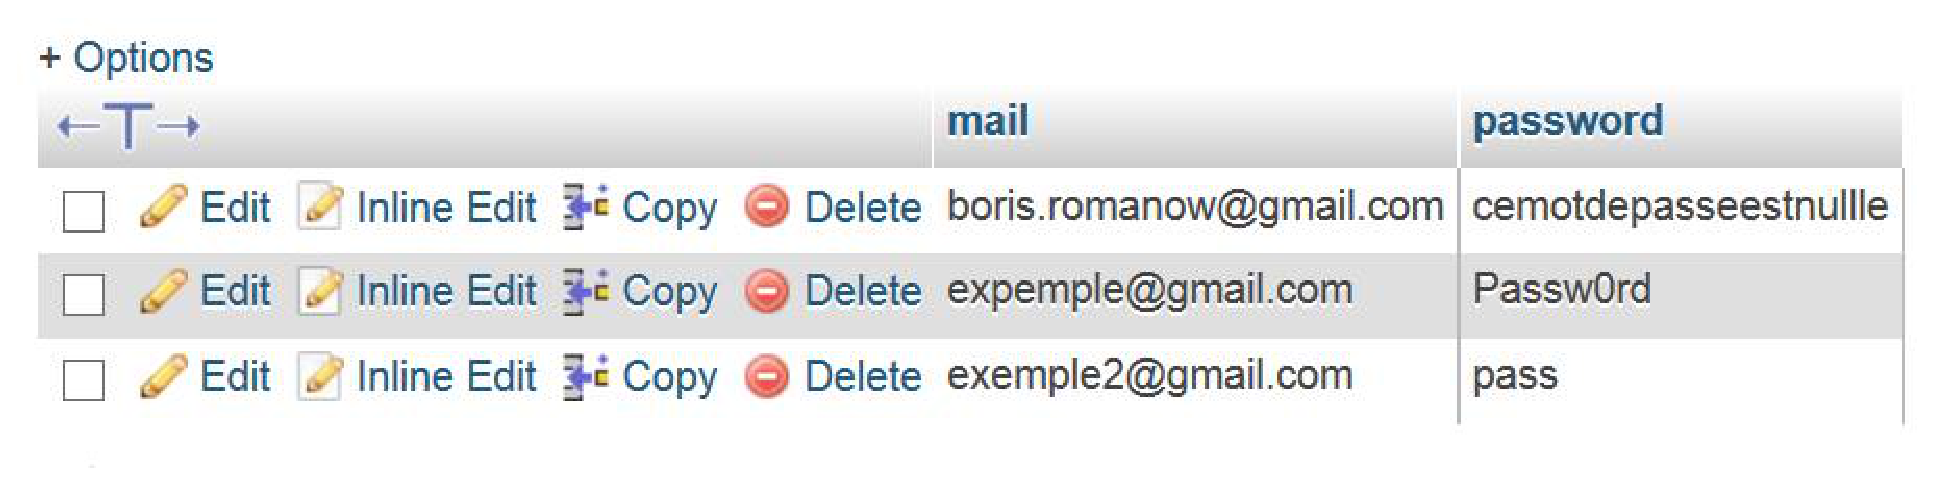
\includegraphics[scale=0.3]{../images/database.eps}
		\caption{PHPMyAdmin database}
		\label{database}
	\end{figure}
\end{frame}

\subsection{Legal testing}
\begin{frame}{What we did to legally test security flaw}
	\begin{itemize}
		\item Work on a personnal WLAN\\
		\item Every test was ran on our personnal machines\\
	\end{itemize}
\end{frame}

\subsection{Counter measures}
\begin{frame}{Counter measures to prevent this kind of attack}
For the website owner : \\
	\begin{itemize}
		\pause \item Avoid HTTP\\
		\pause \item HTTPS certificate\\
	\end{itemize}
\pause For the internet user : \\
	\begin{itemize}
		\pause \item Secured network\\
		\pause \item HTTPS / verified certificate\\
	\end{itemize}
\end{frame}

\section{Encountered problems}
\begin{frame}{Encountered problems}
	\begin{itemize}
		\item What they were.\\
		\item How we actually dealt with them.\\
	\end{itemize}	
\end{frame}

\section{Differences with the Overview's Objectives}
\begin{frame}{Differences with the Overview's Objectives}
	\begin{itemize}
		\item Why did we not met our objectives.\\
		\item What are the possible solutions to meet them.\\
	\end{itemize}
\end{frame}

\section{The End}
\begin{frame}{The End}
	Any questions ?
\end{frame}

\end{document}